\documentclass{llncs}
\usepackage[top=1in, bottom=1in,right=1in,left=1in]{geometry}                % See geometry.pdf to learn the layout options. There are lots.
%\geometry{letterpaper}                   % ... or a4paper or a5paper or ... 
%\geometry{landscape}                % Activate for for rotated page geometry
%\usepackage[parfill]{parskip}    % Activate to begin paragraphs with an empty line rather than an indent
%\usepackage{jcompbio}
\usepackage{graphicx}
\usepackage{amssymb}
\usepackage{amsmath}
%\usepackage{amsthm} %pour les newtheorem
\usepackage{epstopdf}
\usepackage{xspace}
\usepackage{relsize}
\usepackage[numbers]{natbib}
\usepackage[colorinlistoftodos,textsize=small]{todonotes}

\makeatletter
\renewcommand\bibsection%
{
  \section*{\refname
    \@mkboth{\MakeUppercase{\refname}}{\MakeUppercase{\refname}}}
}
\makeatother


%\usepackage{subfig} %Subfigures
%\usepackage{subcaption} %Subfigures

\usepackage{tikz}
\usepackage{amsmath}
\usepackage{ifthen}
\usepackage{relsize}
\usetikzlibrary{positioning}
\usetikzlibrary{matrix}
\usetikzlibrary{calc}
\usetikzlibrary{shapes}
\usetikzlibrary{arrows}
\usetikzlibrary{fit}
\usetikzlibrary{decorations}
\usetikzlibrary{snakes}
\usetikzlibrary{shadows}
\pgfdeclarelayer{background}
\pgfdeclarelayer{backbackground}
\pgfdeclarelayer{foreground}
\pgfsetlayers{backbackground,background,main,foreground}

%!TEX root = main_RNAPyro_JCB.tex

\newcommand{\ourprog}{\texttt{RNA-MoIP}\xspace} 

\usepackage[applemac]{inputenc} %for the encoding 


\newcommand{\RNAmutants}{\texttt{RNAmutants}\xspace}
\newcommand{\RNApyro}{\texttt{RNApyro}\xspace}

\newcommand{\red}[1]{{\color{red}#1}}
\newcommand{\farna}{\texttt{FARNA}\xspace}
\newcommand{\mcfoldmcsym}{\texttt{MC-Pipeline}\xspace}
\newcommand{\mcfold}{\texttt{MC-Fold}\xspace}
\newcommand{\mcsym}{\texttt{MC-Sym}\xspace}
\newcommand{\nast}{\texttt{NAST}\xspace}
\newcommand{\ifoldrna}{\texttt{iFoldRNA}\xspace}
\newcommand{\rnafold}{\texttt{RNAfold}\xspace}
\newcommand{\rnasubopt}{\texttt{RNAsubopt}\xspace}
\newcommand{\rnawolf}{\texttt{RNAwolf}\xspace}
\newcommand{\rnastructure}{\texttt{RNAstructure}\xspace}
\newcommand{\contrafold}{\texttt{contrafold}\xspace}
\newcommand{\unafold}{\texttt{unafold}\xspace}
\newcommand{\rnadd}{\texttt{RNA2D3D}\xspace}
\newcommand{\assemble}{\texttt{assemble}\xspace}
\newcommand{\fred}{\texttt{FR3D}\xspace}
\newcommand{\rnajunction}{\texttt{RNAjunction}\xspace}
\newcommand{\rnamotif}{\texttt{RNAmotif}\xspace}
\newcommand{\treefolder}{\texttt{TreeFolder}\xspace}
\newcommand{\barnacle}{\texttt{BARNACLE}\xspace}
\newcommand{\contextfold}{\texttt{contextfold}\xspace}
%\newcommand{\citep}{\cite}



\newcommand{\Z}[3]{\mathcal{Z}_{#1, #2}^{#3}}
\newcommand{\Y}[3]{\mathcal{Y}_{#1, #2}^{#3}}
\newcommand{\B}{\mathcal{B}}
\newcommand{\Kron}{\delta}

\newcommand{\ub}{\bullet}
\newcommand{\op}{\text{\tt(}}
\newcommand{\cp}{\text{\tt )}}

\newcommand{\Struct}{S}
\newcommand{\BoolFalse}{F}
\newcommand{\BoolTrue}{T}
\newcommand{\N}{{\sf N}}
\newcommand{\gc}{gc}

\newcommand{\PE}[1]{E(#1)}
\newcommand{\EI}{\text{EI}}
\newcommand{\ES}{\text{ES}}
\newcommand{\ISO}{\text{ISO}}

\newcommand{\EBP}[3]{E^{\Omega,\beta}_{(#1),\binom{#3}{#2}}}


\newcommand{\Ab}{{\sf{A}}}
\newcommand{\Cb}{{\sf{C}}}
\newcommand{\Gb}{{\sf{G}}}
\newcommand{\Ub}{{\sf{U}}}


%%%%%%%%%%%% Comments macros %%%%%%%%%%%%%%%%%%%%%

\newcommand{\ShowTODO}[1]{{#1}}
%\renewcommand{\ShowTODO}[1]{}

\newcommand{\TODO}[2]{\ShowTODO{\todo[inline, linecolor=#1, backgroundcolor=#1!60!white,bordercolor=#1]{#2}}}
\newcommand{\Discussion}[1]{\footnote{#1}}

\newcommand{\TODOTous}[1]{\TODO{orange}{{\bf TODO Tous :} #1}}
\newcommand{\TODOJerome}[1]{\TODO{blue!80!white}{{\bf TODO Jerome :} #1}}
\newcommand{\TODOYann}[1]{\TODO{gray}{{\bf TODO Yann :} #1}}
\newcommand{\TODOVlad}[1]{\TODO{green!60!black}{{\bf TODO Vlad :} #1}}

%%%%%%%%%%%%%%% End Comments %%%%%%%%%%%%%%%%%%%%%



\newcommand{\SpaceCheating}{\vspace{-0em}}
\newcommand{\ScaleDP}{.55}

\colorlet{StressColor}{red!60!black}



%\title{An inside-outside algorithms for mutant RNAs with applications to error detections in structured RNAs}
\title{Using structural knowledge to correct RNA pyrosequencing errors in non-coding RNAs}
\author{Vladimir Reinharz\inst{1}, Yann Ponty\inst{2}$^{*}$ \and J\'er\^{o}me Waldisp\"{u}hl\inst{1}$^*$}
\date{}
\institute{School of Computer Science, McGill University, Montreal, Canada.
	\and  Laboratoire d'informatique, \'Ecole Polytechnique, Palaiseau, France.
	 \\\email{jeromew@cs.mcgill.ca}, \email{yann.ponty@lix.polytechnique.fr}}


%Last thing before BEGIN DOC for links to appear in pdf

%  \usepackage{hyperref}
%  \hypersetup{colorlinks}
%              citecolor=black,
%              filecolor=black%
%              linkcolor=black%
%              urlcolor=black%
%              pdftex}


\begin{document}

\ShowTODO{\setcounter{tocdepth}{1}
\listoftodos} 
\maketitle
%\section{}
%\subsection{}
\begin{abstract}
Analysis of the sequence-structure relationship in RNA molecules are essential to evolutionary studies but also to 
concrete applications such as error-correction methodologies in sequencing technologies. The prohibitive sizes of the
mutational and conformational landscapes combined with the volume of data to proceed require efficient algorithms 
to compute sequence-structure properties. More specifically, here we aim to calculate which mutations increase the most the 
likelihood of a sequence to a given structure and RNA family.\\
In this paper, we introduce \RNApyro, an efficient linear-time and space inside-outside algorithm that computes exact mutational
probabilities under secondary structure and evolutionary constraints given as a multiple sequence alignment with a consensus structure.
We develop a scoring scheme combining classical stacking base pair energies to novel isostericity scales, and apply our techniques
to correct point-wise errors in 5s rRNA sequences. Our results suggest that \RNApyro is a promising algorithm to complement existing
tools in the NGS error-correction pipeline. 

\noindent
\textbf{Key words:} RNA, mutations, secondary structure
\end{abstract}

%\newpage

\input{introduction_JCB.tex}

%!TEX root = main_RNAPyro_JCB.tex

\section{Methods}
\label{sec:methods}

We introduce a probabilistic model, which aims at capturing both the stability of the folded RNA and its affinity towards a predefined 3D conformation.
To that purpose, a Boltzmann weighted distribution is assumed, based on a pseudo-energy function $\PE{\cdot}$ which includes contributions for both the free-energy and its putative isostericity towards a multiple sequence alignment. In this model, the probability that the nucleotide at a given position needs to be mutated (i.e. corresponds to a sequencing error) can be computed using a variant of the \emph{Inside-Outside algorithm}~\cite{Lari1990} in time which scales linearly with the sequence length.


\subsubsection{Definitions.}
Let $\B:=\left\{\Ab,\Cb,\Gb,\Ub\right\}$ be the set of nucleotides.
Given an RNA sequence $s\in \B^n$, let $s_i$ be the nucleotide at position $i$. Let $\Omega$ be a set of un-gapped RNA sequences of
length $n$. $\Struct$ is a secondary structure without pseudoknots, denoted by a dot-parenthesis string (well-parenthesized expression with dots). In any such expression, matched parentheses induce and unambiguous set of corresponding positions, associated with base-pairing positions, mediated by hydrogen bonds. It follows that if $(i,j)$ and $(k,l)$ are base pairs in $S$, there is no overlapping extremities  $\{i,j\}\cap \{k,l\}=\varnothing$ and either the intersection is empty 
 ($[i,j]\cap[k,l]=\varnothing$) or one is included in the other ($[k,l]\subset[i,j]$ or 
 $[i,j]\subset[k,l])$. Let us finally denote by $\delta: \B^*\times \B^* \to \mathbb{N}^+$ the Hamming distance, i.e. the number of differing positions between two sequences $s'$ and $s''$ such that $|s'|=|s''|$.
\TODOYann{Move above, define secondary structure and add fancy VARNA illustration}




\subsection{Probabilistic Model}
Let $\Omega$ be an gap-free RNA alignment sequence, $S$ its associated secondary structure, 
then any sequence $s$ has probability proportional to its Boltzmann factor
\begin{align*}
  {B}(s) &= e^\frac{-\PE{s}}{RT}, &&\text{with}&\PE{s}&:=\alpha\cdot\ES(s,S)+(1-\alpha)\cdot\EI(s,S,\Omega),
\end{align*}
where $R$ is the Boltzmann constant, $T$ the temperature in Kelvin, $\ES(s)$ and $\EI(s,S,\Omega)$ 
are the free-energy and isostericity contributions respectively (further described below), and $\alpha\in[0,1]$ is an arbitrary parameter that sets the relative weight for both contributions.

\subsubsection{Energy Contribution.}
The free-energy contribution in our pseudo-energy model corresponds to an additive stacking-pairs model, using values from the Turner 2004 model retrieved from the NNDB~\cite{Turner2010}. Given a candidate sequence $s$ for a secondary structure $S$, the free-energy of $S$ on $s$ is given by
\begin{align*}
  \ES(s,S) = \sum_{\substack{(i,j)\to (i',j')\in S\\ \text{stacking pairs}}}\ES^{\beta}_{s_is_j\to s_{i'}s_{j'}} 
\end{align*}
where $\ES^{\beta}_{ab\to a'b'}$ is set to $0$ if $ab=\varnothing$ (no base-pair to stack onto), the tabulated free-energy of stacking pairs $(ab)/(a'b')$ in the Turner model if available, or $\beta\in[0,\infty]$ for non-Watson-Crick/Wobble entries (i.e. neither $\Gb\Ub$, $\Ub\Gb$, $\Cb\Gb$, $\Gb\Cb$, $\Ab\Ub$ nor $\Ub\Ab$). This latter parameter allows to choose whether to simply penalize invalid base pairs, or forbid them altogether ($\beta = \infty$).
The loss of precision due to this simplification of the Turner model remains reasonable since the targeted secondary structure is fixed. For instance, multiloops do not consider base-specific contributions, and therefore their consideration would constitute a criterion for preferring a sequence over another. Furthermore, it greatly eases the design and implementation of dynamic-programming equations. 
\subsubsection{Isostericity Contribution.}
The concept of isostericity score~\cite{Stombaugh2009} is based on the geometric discrepancy (superimposability) of two base-pairs, using individual additive contributions computed by Stombaugh~\emph{et al}~\cite{Stombaugh2009}. Let $s$ be a candidate sequence for a secondary structure $S$, given in the context of a gap-free RNA alignment $\Omega$,  we define the isostericity contribution to the pseudo-energy as
\begin{align*}
  \ES(s,S,\Omega) &= \sum_{\substack{(i,j)\in S\\ \text{pairs}}}\EI^{\Omega}_{(i,j),s_i s_j}, & \text{where}&& 	\EI^{\Omega}_{(i,j),ab}:=
	\frac{
		\sum_{s'\in\Omega}
			\text{\ISO}((s_i',s_j'),(a,b))}
%-		\left(			\text{\ISO}((s_i',s_j'),(s_i,s_j))				\right)	
{		
		|\Omega|
	}
\end{align*}
is the average isostericity of a base-pair in the candidate sequence, compared with the reference alignment.
The $\ISO$ function uses the {Watson-Crick/Watson-Crick} cis isostericity matrix computed by Stombaugh~\emph{et al}~\cite{Stombaugh2009}. Isostericity scores range between $0$ and $9.7$, $0$ corresponding to a perfect isostericity, and a penalty of $10$ is used for missing entries.
The isostericity contribution exponentially favors sequences that are likely to adopt a similar local conformation as the sequences contained in the alignment.
\TODOYann{Avoid duplicate reference to Stombaugh et al}

\subsubsection{Combining contributions.}
Let us remark that any of the individual contributions can be associated to (a subset of) the base-pairs occurring in the structure, possibly complemented, in the case of stacking pairs, with the knowledge of flanking base-pairing nucleotide.
Therefore, let us denote by $\EBP{i,j}{xy}{a'b'}$ the local contribution of a base-pair $(i,j)$ of nucleotides $(a',b')$, surrounded by a stacking pair $(x,y)$ (or $\varnothing$ otherwise), to the pseudo-energy:
\begin{equation}
  \EBP{i,j}{xy}{a'b'}  = \alpha \cdot\ES^\beta_{xy \to a' b'}+(1-\alpha)\cdot\EI^{\Omega}_{(i,j),a'b'}.
\end{equation}

\subsection{Computing the Mutational Profile of Sequences}


Let $s$ be an RNA sequence, $S$ a reference structure, and $m\geq 0$ a desired number of mutations. 
We are interested in  the probability that a given position contains a specific nucleotide, over all sequences having at most $M$ mutations from $s$
%  under the SCFG derivation $S$ 
(formally $\mathbb{P}(s_i = x\mid s,\Omega, \Struct,M)$). 
We define a variant of the
 \emph{Inside-Outside algorithm}~\cite{Lari1990} to compute this
 probability, based on two sets of dynamic programming equations. 
%from the two  functions $\mathcal{Z}_*^*$ and $\mathcal{Y}_*^*$. 

The former, defined in Equations~\eqref{eq:Z_in} and~\eqref{eq:Z_rec_A}-\eqref{eq:Z_rec_C}, is analogous to an \emph{inside} computation. Considering an interval of the sequence/secondary structure, it consists in the accumulated contributions of any possible sequences that have suitable Hamming distance within the interval. It is therefore similar to a partition function, i.e. the sum of Boltzmann factors over all sequences within $[i,j]$, 
knowing that position $i-1$ is composed of nucleotide $a$ (resp. $j+1$ is $b$), within 
$m$ mutations of $s$. The latter, defined by Equations~\eqref{eq:Y_in} and~\eqref{eq:Y_rec},
 computes the \emph{outside} algorithm,   
the partition function over sequences within $m$ mutations of $s$ outside the interval (restricted to two intervals $[0,i]\cup[j,n-1]$), 
knowing  that flanking inner positions $(i+1,j-1)$ contain nucleotides $a$ and $b$ respectively. A suitable multiplicative combination of these terms, computed as shown in Equation~\eqref{eq:combine}, gives the total weight of every possible sequences that support a given base-pair (or unpaired position) and, in turn, the probability of seeing a specific base at a given position.

%Drawing a parallel with stochastic context-free grammars (SCFG), for which the inside-outside algorithm was introduced, the set of sequences can be seen as the language of words having length $n$, generated from a stochastic context-free grammar.
%These rules would limit the number of mutations (i.e. )
% $S$ can be considered as constraining weighing on the shape of parse trees the derivations in a classic 
% of the {SCFG} generating  all  secondary structures of length  $|s|$. 




\subsubsection{Inside computation.}
\begin{figure}[t]\centering
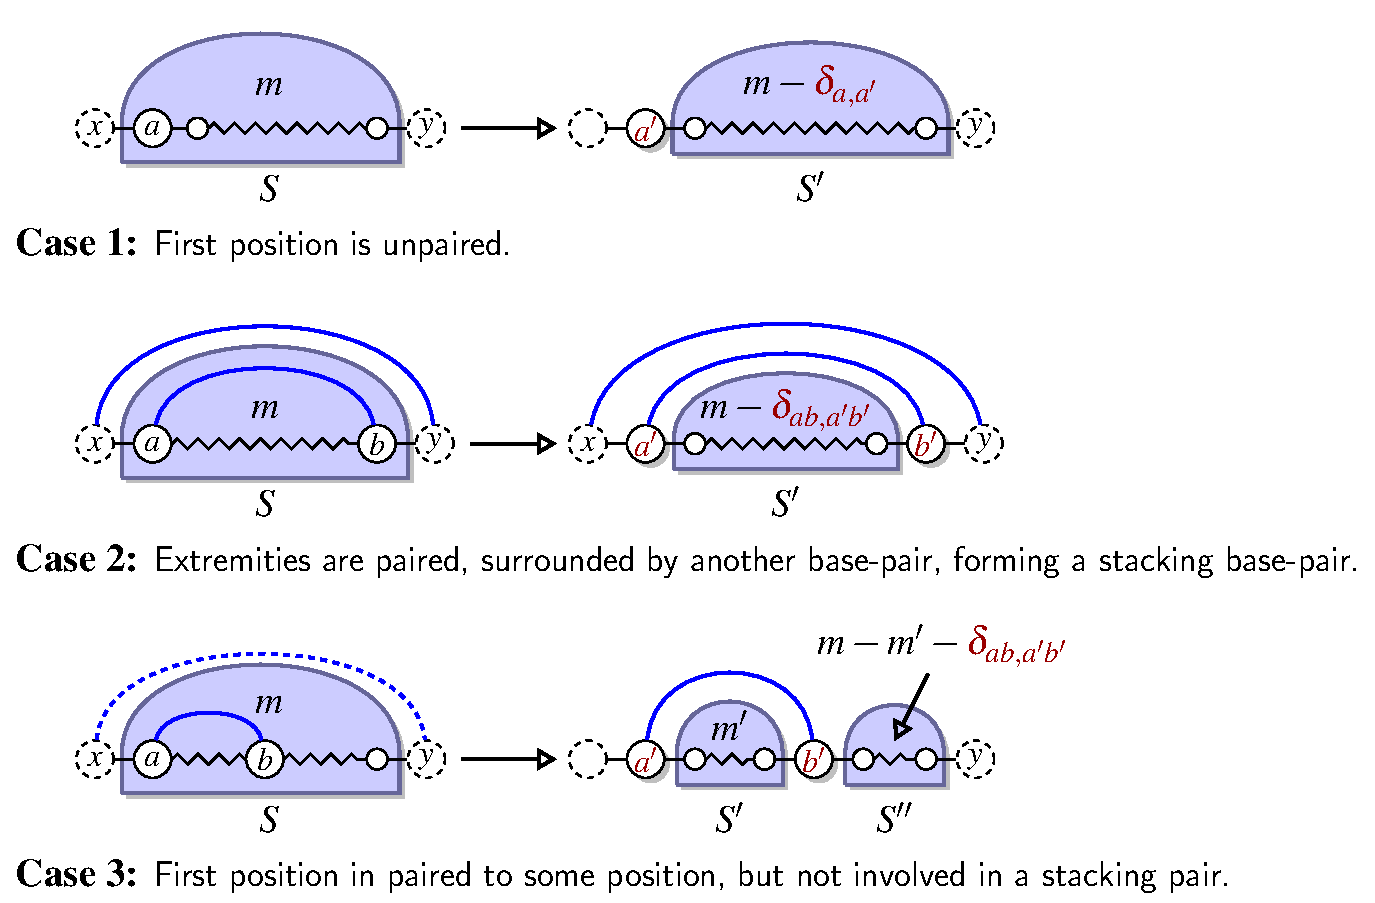
\includegraphics[scale=\ScaleDP]{FigDPInsideWrapper}
\caption{Principle of the inside computation (partition function). Any sequence (mutated)  
can be decomposed as a sequence preceded by a, possibly mutated, base 
(Unpaired case), a sequence surrounded by some base-pair (Stacking-pair case), 
or as two sequences segregated by some base-pair (General base-pairing case). In this latter case, mutations must be distributed between sub-sequences.\label{fig:inside}}
\end{figure}

The \emph{Inside} function $\Z{\Struct}{m}{x,y}$ is simply the partition function, i.e. the sum of Boltzmann factors over all sequences for a substructure $\Struct$ (implicitly attached to an interval $[i,j]$ of the sequence), featuring $m$ mutations/errors compared to $s$, and having flanking nucleotides $x$ and $y$. 
Such terms can be computed by recurrence, using the following equation for the initial case:
\begin{equation}
	\forall x,y\in B\times \B, m\in [0,M]:\, \Z{\varepsilon}{m}{x,y}=\left\{
	\begin{array}{ll}
		1 &\text{ If } m = 0\\
		0 &\text{ Otherwise.}
	\end{array}\right.
\label{eq:Z_in}
\end{equation}
In other words, either there is no sequence at distance $m>0$ of the empty sequence, or the only allowed sequence is the empty sequence ($m=0$), having energy $0$. Since the contributions only depend on base pairs, they do not appear in the initial conditions. 

The main recursion considers a general structure $\Struct$, flanked by two nucleotides (outside the region of interest) $x$ and $y$, respectively on the $5'$ and $3'$ end of the sequence. As illustrated by Figure~\ref{fig:inside}, it is computed, for each subinterval $[i,j]$, by considering one of the three following cases, dependent on the base-pairing status and context of the leftmost position in the sequence/structure:
\begin{itemize}
\item {\bf Case 1: Unpaired leftmost position.} If the first position  is unpaired in the structure, then $\Struct$ can be further decomposed, using a dot-parenthesis notation, as $\Struct = \ub \Struct'$. Let $a\in B$ be the nucleotide found at the leftmost position in the initial structure, then one has:
\begin{equation}
\label{eq:Z_rec_A}
	\Z{\Struct}{m}{x,y} =
      \sum_{\substack{a'\in \B,\\ \Kron_{a,a'}\le m}}  
      \Z{\Struct'}{m-\Kron_{a,a'}}{a',y}.
\end{equation}
Indeed, any suitable sequence is a concatenation of a, possibly mutated, nucleotide $a'$ at the first position, followed by a sequence over the remaining interval, having $m-\Kron_{a,a'}$ mutations (accounting for a possible mutation at first position), and having flanking nucleotides $a'$ and $y$.
\item {\bf Case 2: Paired ends, stacking onto another base-pair.} If both ends of the considered interval form a base-pair ($\Struct = \op\Struct'\cp$), stacking onto another base pair just outside whole region, then the isosteric contribution of the base-pair must be supplemented with a specific "stacking-pairs" bonus. Let $a$ and $b$ be the nucleotides found on both ends of the interval (positions $i$ and $j$), then one has
\begin{equation}
\label{eq:Z_rec_B}
	\Z{\Struct}{m}{x,y} =
      \sum_{\substack{a',b'\in \B^2,\\ \Kron_{ab,a'b'}\le m}}
			 e^{\frac{-\EBP{i,j}{xy}{a'b'}}{RT}}
			 \cdot \Z{S'}{m-\Kron_{ab,a'b'}}{a',b'}.
\end{equation}
Any sequence generated here consists of two, possibly mutated, nucleotides $a'$ and $b'$, flanking a sequence over the remaining portion. In order for the total distance to sum to $m$, this portion must feature $m-\Kron_{ab,a'b'}$ additional point wise mutations.

\item {\bf Case 3: Paired leftmost position, but no stacking pairs.} In this case, the structure is split into two parts by the base pair ($\Struct = \op \Struct'\cp\Struct''$). Let us denote by $k$ the partner of position $i$, and by $a$, $b$ and $c$ the bases found at positions $i$, $k$ and $j$ respectively, then one has:
\begin{equation}
\label{eq:Z_rec_C}
	\Z{\Struct}{m}{x,y}=\sum_{\substack{a',b'\in \B^2,\\ \Kron_{ab, a'b'}\le m}}
      \sum_{m'=0}^{m-\Kron_{ab,a'b'}}
   		 e^{\frac{-\EBP{i,k}{\varnothing}{a'b'}}{RT}}
      \cdot\Z{\Struct'}{m-m'-\Kron_{ab,a'b'}}{a',b'}
      \cdot\Z{\Struct''}{m'}{b',y}.
\end{equation}
In other words, if the leftmost position is paired, and the base-pair is not stacking onto another base-pair, then the  only term contributing directly to the energy is the isostericity of the base pair. Admissible sequences for $\Struct$ consist of two paired nucleotides $a'$ and $b'$ at positions $i$ and $k$ respectively, flanking a sequence for $\Struct'$ (over an interval $[i+1,k-1]$), and followed by a (possibly empty) sequence for $\Struct''$ (over $[k+1,j]$). Since the total number of mutations sums to $m$, a parameter $m'$ is introduced to distribute the remaining mutations between the two sequences.
\end{itemize}


\subsubsection{Outside computation.}	
\begin{figure}[t]\centering
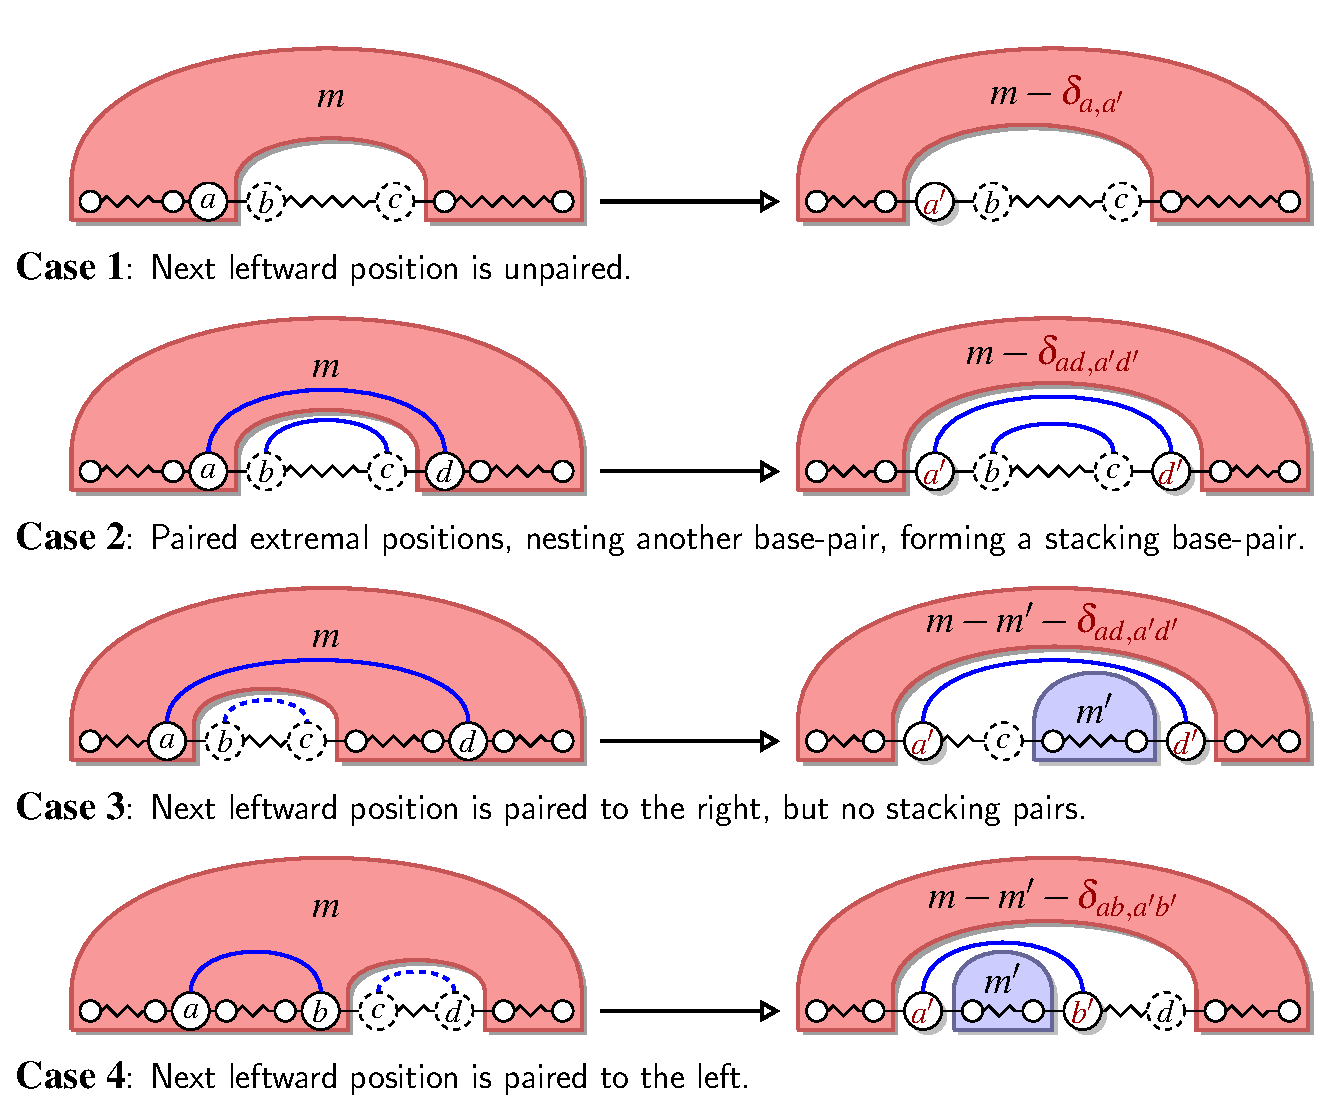
\includegraphics[scale=\ScaleDP]{FigDPOutsideWrapper}
\caption{Principle of the outside computation. Note that the outside algorithm uses intermediate results from the inside algorithm, 
therefore its efficient implementation requires a precomputation of the inside contributions.}
\end{figure}

The \emph{Outside} function, $\Y{\Struct}{m}{x,y}$ is the partition function considering only the 
contributions of subsequences excluding a given structure/interval $\Struct$, occupying the open interval $]i,j[$ in the sequence, at Hamming distance exactly $m$ to the initial sequence $s$, and assuming that nucleotides $x$ and $y$ were previously chosen for $i+1$ and $j-1$, the outermost portions of the excluded structure.
\TODOYann{Reformat outside Figure as in Incarnation.}
The associated terms $\Y{\Struct}{m}{x,y}$ can then be computed recursively, considering as the base case any prefix $\Struct$ of the complete structure:
\begin{equation}
	\forall x,y\in B\times \B, \forall \Struct'\text{ s.t. }\Struct=\Struct'.\Struct'', m\in [0,M]:\, \Y{\Struct^\ast}{m}{x,y}=\Z{\Struct''}{m}{y,X}
\label{eq:Y_in}
\end{equation}
where $X\in\B$ can be any nucleotide, and will not affect further computations.

The main recurrence below extends the excluded structure leftward, and considers four cases depending on its base-pairing status and directionality:
\begin{itemize}
\item {\bf Case 1: Unpaired position.}
\begin{equation}
	\Y{\Struct}{m}{x,y} = \sum_{\substack{a'\in \B,\\ \Kron_{a,a'}\le m}}
    \Y{\ub\Struct}{m- \Kron_{a,a'}}{a',y}
\label{eq:Y_rec_A}
\end{equation}
\item {\bf Case 2: Stacking base-pair.}
\begin{equation}
	\Y{\Struct}{m}{x,y} = 
    \sum_{\substack{a'b'\in \B^2,\\ \Kron_{ab,a'b'}\le m}}
		 e^{\frac{-\EBP{i,j}{xy}{a'b'}}{RT}}\cdot
    \Y{\op\Struct\cp}{m- \Kron_{ab,a'b'}}{a',b'} 
\label{eq:Y_rec}
\end{equation}
\item {\bf Case 3: Next position paired rightward.}
\begin{equation}
	\Y{i,j}{m}{a,b} = \sum_{\substack{a'b'\in \B^2,\\ \Kron_{a'b',s_is_k}\le m}}
		 \sum_{m'=0}^{m-\Kron_{a'b',s_is_k}}
  		 e^{\frac{-E_{(i,k),\varnothing\to a'b'}^{\Omega,\beta}}{RT}}
		 \cdot\Y{i-1,k+1}{m- \Kron_{a'b',s_is_k} - m'}{a',b'}
     \cdot\Z{j,k-1}{m'}{b,b'} 
\label{eq:Y_rec}
\end{equation}
\item {\bf Case 4: Next position paired leftward.}
\begin{equation}
	\Y{i,j}{m}{a,b} = 
		 \sum_{\substack{a'b'\in \B^2,\\ \Kron_{a'b',s_ks_i}\le m}}
		 \sum_{m'=0}^{m-\Kron_{a'b',s_ks_i}}
   	 e^{\frac{-E_{(k,i),\varnothing\to a'b'}^{\Omega,\beta}}{RT}}
		 \cdot\Y{k-1,j}{m- \Kron_{a'b',s_ks_i} - m'}{a',b}
     \cdot\Z{k+1,i-1}{m'}{a',b'}
\label{eq:Y_rec}
\end{equation}
\end{itemize}
\TODOYann{Rephrase in term of tree, as in Incarnation??}
The five cases can be broked down as follows.
\begin{description}
\item[$S_i=-1$:] If the nucleotide at position $i$ is not paired, then the value is the same
as if we decrease the lower interval bound by $1$ (i.e. $i-1$), and consider all possible
nucleotides $a'$ at position $i$, correcting the number of mutants
in function of $\Kron_{a',s_i}$.
\item[$S_{i}=j$ and $S_{i+1}=j-1$:] If nucleotide $i$ is paired with $j$ and nucleotide $i+1$ is
paired with $j-11$, we are in the only case were stacked base pairs can occur. We thus add
the energy of the stacking and of the isostericity of the base pair $(i,j)$. What is left
to compute is the \emph{outside} value for the interval $[i-1,j+1]$ over all possible nucleotides 
$a',b'\in B^2$ at positions $i$ and $j$ respectively.
\item[$S_{i}=k \geq j$:]If nucleotide $i$ is paired with position $k\geq j$, 
and is not stacked inside, the 
only term contributing directly to the energy is the isostericity of base pair $(i,k)$. 
Therefore, we consider the outside interval $[i-1,k+1]$, multiplying it by the \emph{inside}
value of the newly included interval (i.e. $[j,k-1]$), for 
all possible values $a',b'\in B^2$ for nucleotides at positions $i$ and $k$ respectively.
\item[$-1<S_{i}<i$:]As above but if position $i$ is paired with a lower value.
\item[Else:] Any other derivation of the SCFG does not correspond to the 
secondary structure $S$, and we return $0$.


\end{description}

\subsubsection{Combining Inside and Outside Values into Point-Wise Mutations Probabilities.}
By construction, the partition function over all sequences at exactly $m$ mutations of a reference sequence $s$ can 
be either described from the \emph{inside} contribution $\Z{0,n-1}{m}{X,X}$ of the whole sequence,
$\forall X\in B$, or from \emph{outside} terms as:
$$
	\Z{0,n-1}{m}{X,X}
	\equiv
	\sum_{\substack{a\in \B,\\ \Kron_{a,s[k]}\le m}}	
	\Y{k-1,k+1}{m-\Kron_{a,s[k]}}{a,a},\forall k \text{	unpaired.}
$$

We are now left to compute the probability that a given position is a given nucleotide.
We leverage the \emph{Inside-Outside} construction to immediately obtain the following $3$ cases.
Given $i\in[0,n-1],x\in B$, and $M\geq 0$ a bound on the number of allowed mutations, one defines
\begin{equation}
	\mathbb{P}(s_i = x\;|\; M) := \frac{\mathcal{W}^M_{\substack{i, [x]}}}{\sum_{m=0}^{M}\Z{0,n-1}{m}{X,X}}\label{eq:normalize}
\end{equation}
where $\mathcal{W}{\substack{\ast\\ \ast}}$ is defined by:
\begin{equation}
\resizebox{\textwidth}{!}{%
$ \mathcal{W}^M_{\substack{i, [x]}} =  \left\{
	\begin{array}{ll}
			\sum_{m=0}^{M}
			\Y{i-1,i+1}{m-\Kron_{x,s_i}}{x,x}
		&\text{If }S_i = -1\\
			\displaystyle
			\sum_{m=0}^{M}
			\sum_{\substack{b\in B\\\Kron_{xb,s_is_k\leq m}}}
			\sum_{m'=0}^{m-\Kron_{xb,s_is_k}}
     	 e^{\frac{-E_{(i,k),\varnothing\to xb}^{\Omega,\beta} }{RT}}
			\cdot\Y{i-1,k+1}{m-\Kron_{xb,s_is_k-m'}}{x,b}
			\cdot\Z{i+1,k-1}{m'}{x,b}
		&\text{If }S_i=k>i\\
    \displaystyle
			\sum_{m=0}^{M}
			\sum_{\substack{b\in B\\\Kron_{bx,s_ks_i\leq m}}}
			\sum_{m'=0}^{m-\Kron_{bx,s_ks_i}}
     	 e^{\frac{-E^{\Omega, \beta}_{(k,i),\varnothing\to bx}}{RT}}
			\cdot\Y{k-1,i+1}{m-\Kron_{bx,s_ks_i-m'}}{b,x}
			\cdot\Z{k+1,i-1}{m'}{b,x}
		&\text{If }S_i=k<i
	\end{array}\right.
$}\label{eq:combine}
\end{equation}

\TODOYann{Rephrase as tree constructs}
\TODOVlad{Add illustration of Inside/Outside combination (adapted from RECOMB presentation??)}
In every case, the denominator is the sum of the partitions function of exactly $m$ mutations, 
for $m$ smaller or equal to our target $M$. The numerators are divided in the following three cases.
\begin{description}
\item[$S_i=-1$:] If the nucleotide at position $i$ is not paired, we are concerned by the weights
over all sequences which have at position $i$ nucleotide $x$, which is exactly the sum
of the values of $\Y{i-1,i+1}{m-\Kron_{x,s_i}}{x,x}$, for all $m$ between $0$ and $M$.
\item[$S_i=k>i$:] Since we need to respect the derivation of the secondary structure $S$, if 
position $i$ is paired, we must consider the two partition functions. The \emph{outside} of the 
base pair, and the \emph{inside}, for all possible values for the nucleotide at position $k$, and
all possible distribution of the mutant positions between the inside and outside of the base pair. We also add the term of isostericity for this specific base pair.
\item[$S_i=k<i$:] Same as above, but with position $i$ pairing with a lower position.
\end{description}

\subsection{Complexity Considerations}
Equations~\eqref{eq:Z_rec} and~\eqref{eq:Y_rec} can be computed using dynamic programming. Namely, the $\mathcal{Z}^{*}_{*}$ and $\mathcal{Y}^{*}_{*}$ terms are computed starting from smaller values of $m$ and interval lengths, memorizing the results as they become available to ensure constant-time access during later stages of the computation. Furthermore, energy terms $E(\cdot)$ can be accessed in constant time thanks to a simple precomputation (not described)  of the isostericity contributions in $\Theta(n\cdot|\Omega|)$. Computing any given term therefore requires $\Theta(m)$ operations.

In principle, $\Theta(m\cdot n^2)$ terms, identified by $(m,i,j)$ triplets, should be computed.
However, a close inspection of the recurrences reveals that the computation can be safely restricted to a subset of intervals $(i,j)$.
For instance, the inside algorithm only requires computing intervals $[i,j]$ that do not break any base-pair, and whose next position $j+1$ is either past the end of the sequence, or is base-paired prior to $i$. Similar constraints hold for the outside computation, resulting in a drastic limitation of the combinatorics of required computations, dropping from $\Theta(n^2)$ to $\Theta(n)$ the number of terms that need to be computed and stored. Consequently the overall complexity of the algorithm is $\Theta(n\cdot(|\Omega|+m^2))$ arithmetic operations and $\Theta(n\cdot(|\Omega|+m))$ memory.


%!TEX root = main_RNAPyro_JCB.tex
\section{Results}
\label{sec:results}

\subsection{Implementation}
The software was implemented in Python2.7 using the \textit{mpmath}~\cite{mpmath} library
for  arbitrary floating point precision. The source code is freely available at:

{\centering \url{https://github.com/McGill-CSB/RNApyro}\\}

The time benchmarks were performed on a MacMini 2010, 2.3GHz dual-core Intel Core i5, 8GB of RAM.
Since typical use-cases of \RNApyro require
 efficiency and scalability, we present in Table~\ref{tab:time} typical runtimes required to compute the probabilities for  every nucleotide at every positions for a vast set of parameters. For those tests,
 both the sequences and the target secondary structure were generated at random.
\TODOVlad{Add more extensive time benchmark, as a plot}


\begin{table}[t]
\begin{minipage}{.4\textwidth}
\begin{tabular}{rccc}
Length &\multicolumn{3}{c}{\#mutations}\\\cline{2-4}
		 			  & 6   &  12  & 24\\\cline{2-4}
100  				& 35s  & 238s & 1023s\\
300  			& 135s & 594s &2460s\\\cline{2-4}
		 						& 25   &    &	50		\\\cline{2-4}
500         & 5400s&       &  21003s    \\
\end{tabular}
\end{minipage}
\begin{minipage}{.59\textwidth}
\caption{Time required by the computation of probabilities. First column indicates the length and  the column indexes indicate the number
 of mutations. $\alpha$ is
set at $0.5$,  $\beta$ to $15$ and $|\Omega|=44$.}
\label{tab:time}
\end{minipage}
\SpaceCheating
\end{table}


\subsection{Error Correction in 5s rRNAs}

To illustrate the potential of our algorithm, we applied our techniques to identify and correct point-wise errors in RNA sequences
with conserved secondary structures. More precisely, we used \RNApyro to reconstruct 5s rRNA sequences with randomly distributed
mutations. This experiment has been designed to suggest further applications to error-corrections in pyrosequencing data.

We built our data set from the 5S rRNA multiple sequence alignment (MSA) available in the Rfam Database 11.0 (Rfam id: \texttt{RF00001}).
Since our software does not currently implement gaps (mainly because scoring indels is a challenging issue that cannot be fully addressed
in this work),  we clustered together the sequences with identical gap locations. From the $54$ MSAs without gap produced, we selected the
biggest MSA  which contains $130$ sequences (out of $712$ in the original Rfam MSA). Then, in order to avoid overfitting, we used \texttt{cd-hit}
\cite{Li:2006fk} to remove sequences with more than 80\% of sequence similarity. This operation resulted in a data set of $45$ sequences. 

We designed our benchmark using a leave-one-out strategy. We randomly picked a single sequence from our data set and performed $12$ random
mutations, corresponding to an error-rate of 10\%. We repeated this operation $10$ times. The value of $\beta$ was set to $15$ (larger values gave similar results). 
To estimate the impact on the distribution of the relative weights of energy and isostericity, we used 4 different values of $\alpha = {0, 0.5, 0.8, 1.0}$. 
Similarly, we also investigated the impact of an under- and over- estimate of the number of errors, by setting the presumed number of errors to 50\% (6 mutations) and 200\% (24 mutations) of their exact number (i.e. $12$).

To evaluate our method, we computed a ROC curve representing the performance of a classifier based on the mutational probabilities computed
by \RNApyro. More specifically, we fixed a threshold $\lambda \in [0,1]$, and predicted an error at position $i$ in sequence $\omega$ if and only if the
probability $P(i,x)$ of a nucleotide $x \in \{ A,C,G,U \}$ exceeds this threshold. To correct the errors we used the set of nucleotides having probability
greated than $\lambda$, that is  $C(i) = \{ x \; | \;  x \in \{ A,C,G,U \} \mbox{ and } P(i,x) > \lambda \mbox{ and }  n \neq \omega[i] \},$ where $\omega[i]$ is
the nucleotide at position $i$ in the input sequence. We note that, for lower thresholds, multiple nucleotides may be available in $C(i)$ to correct
the sequence. Here, we remind that our aim is to estimate the potential of error-correction of \RNApyro, and not to develop a full-fledged error-correction pipe-line, which  
shall be the subject of further studies. Finally, we progressively varied $\lambda$ between $0$ and $1$ to calculate the ROC curve and the area
under the curve (AUC). Our results are reported in Figure~\ref{fig:ROCall}. 

\begin{figure}
\centering
	\includegraphics[width=\textwidth]{subfigs_perform.png}\\

%\begin{subfigure}[b]{0.3\textwidth}
%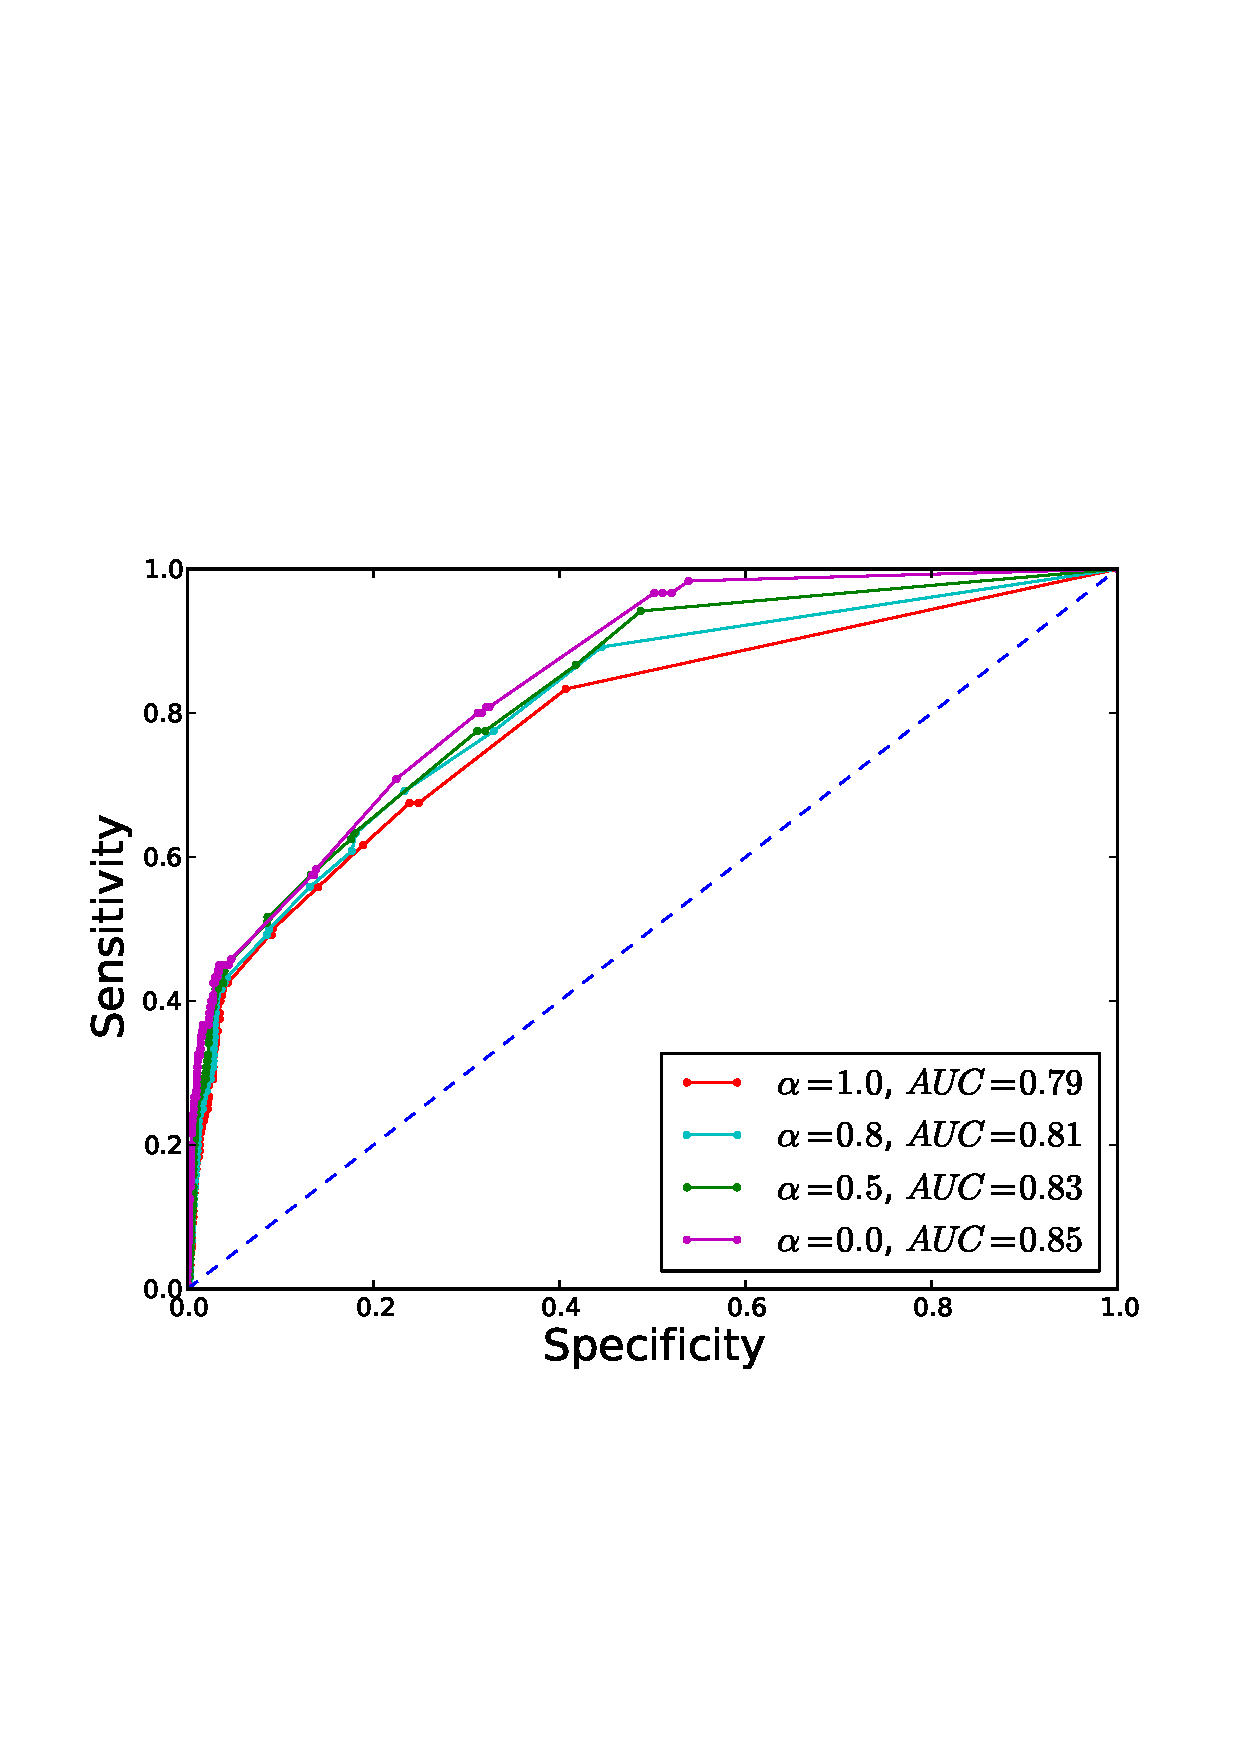
\includegraphics[width=1.2\textwidth]{figures/ROC_6.pdf}
%\caption{6 mutations}
%\label{fig:ROC6mut}
%\end{subfigure}
%\hfill
%\begin{subfigure}[b]{0.3\textwidth}
%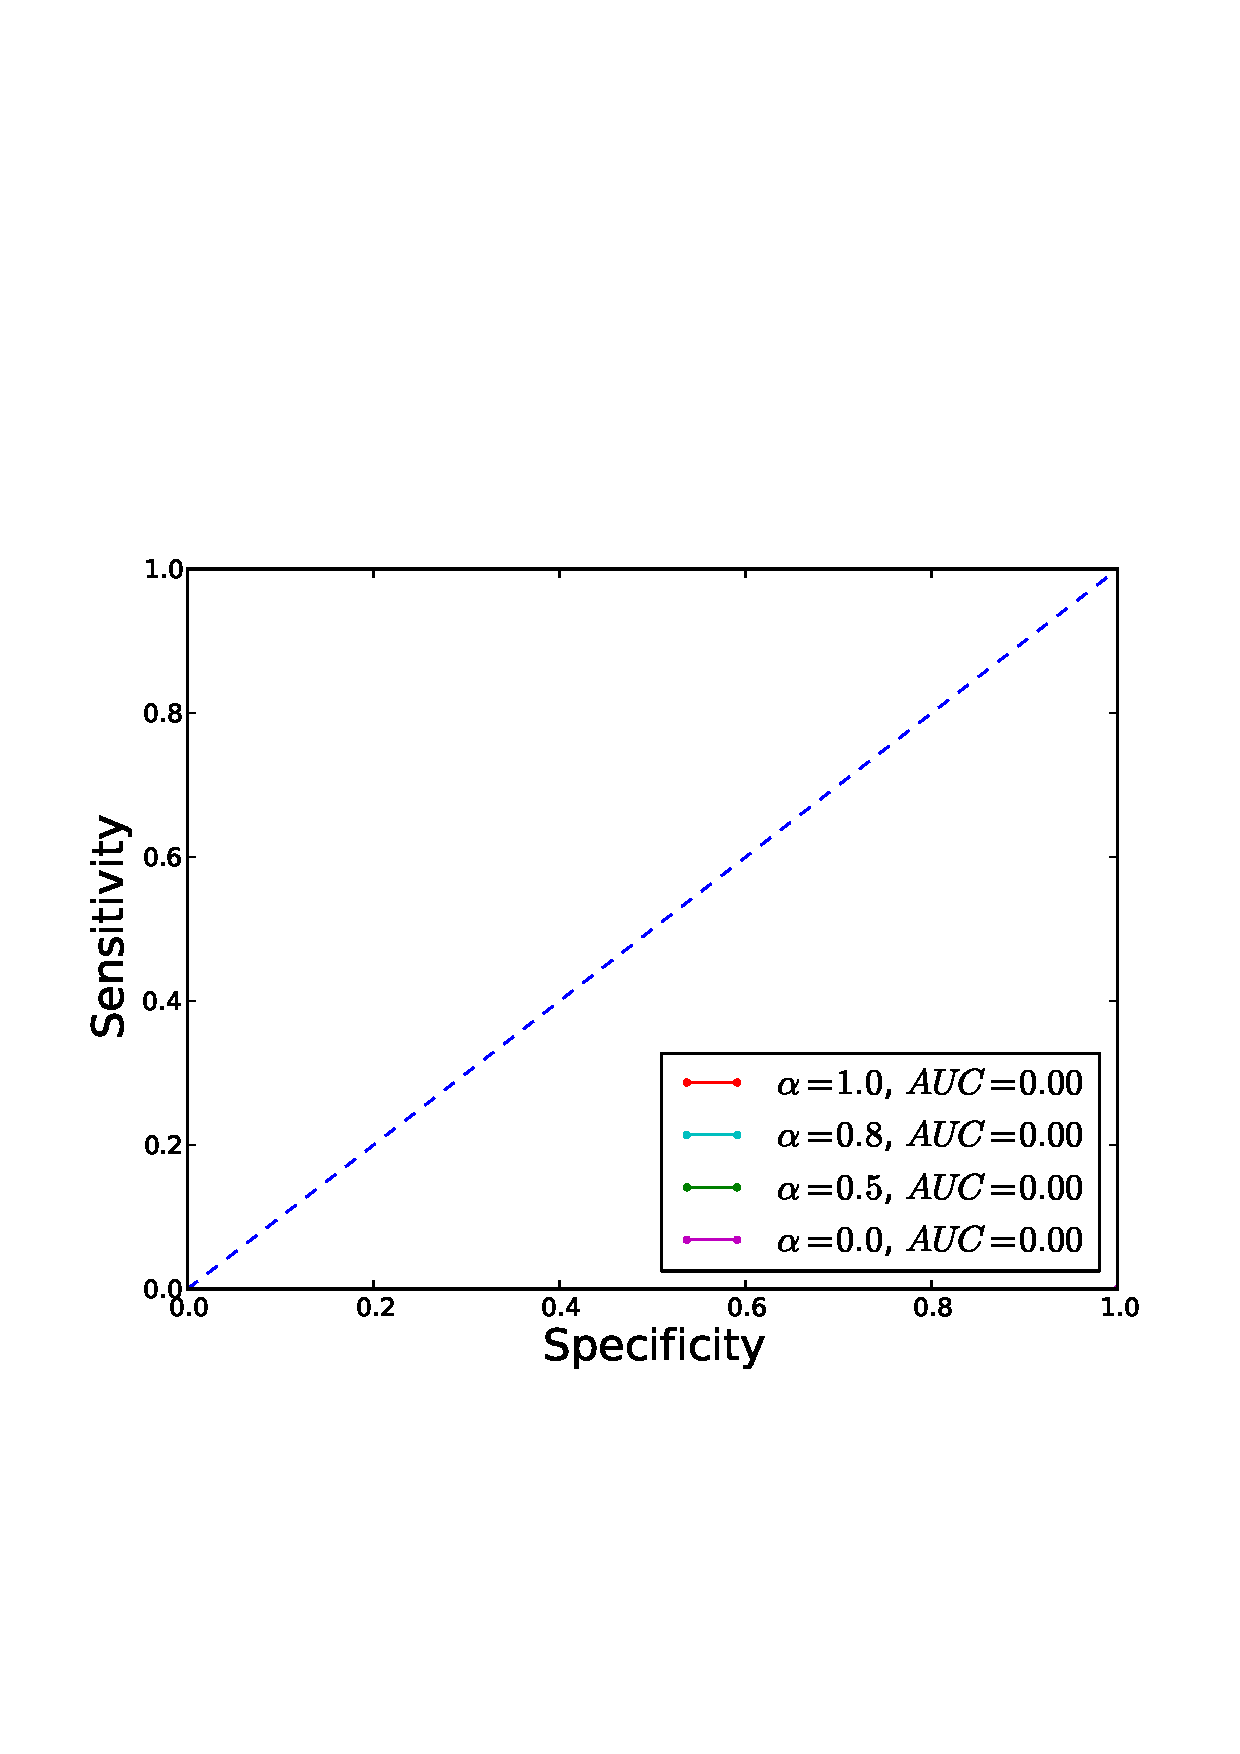
\includegraphics[width=1.2\textwidth]{figures/ROC_12.pdf}
%\caption{12 mutations}
%\label{fig:ROC12mut}
%\end{subfigure}
%\hfill
%\begin{subfigure}[b]{0.3\textwidth}
%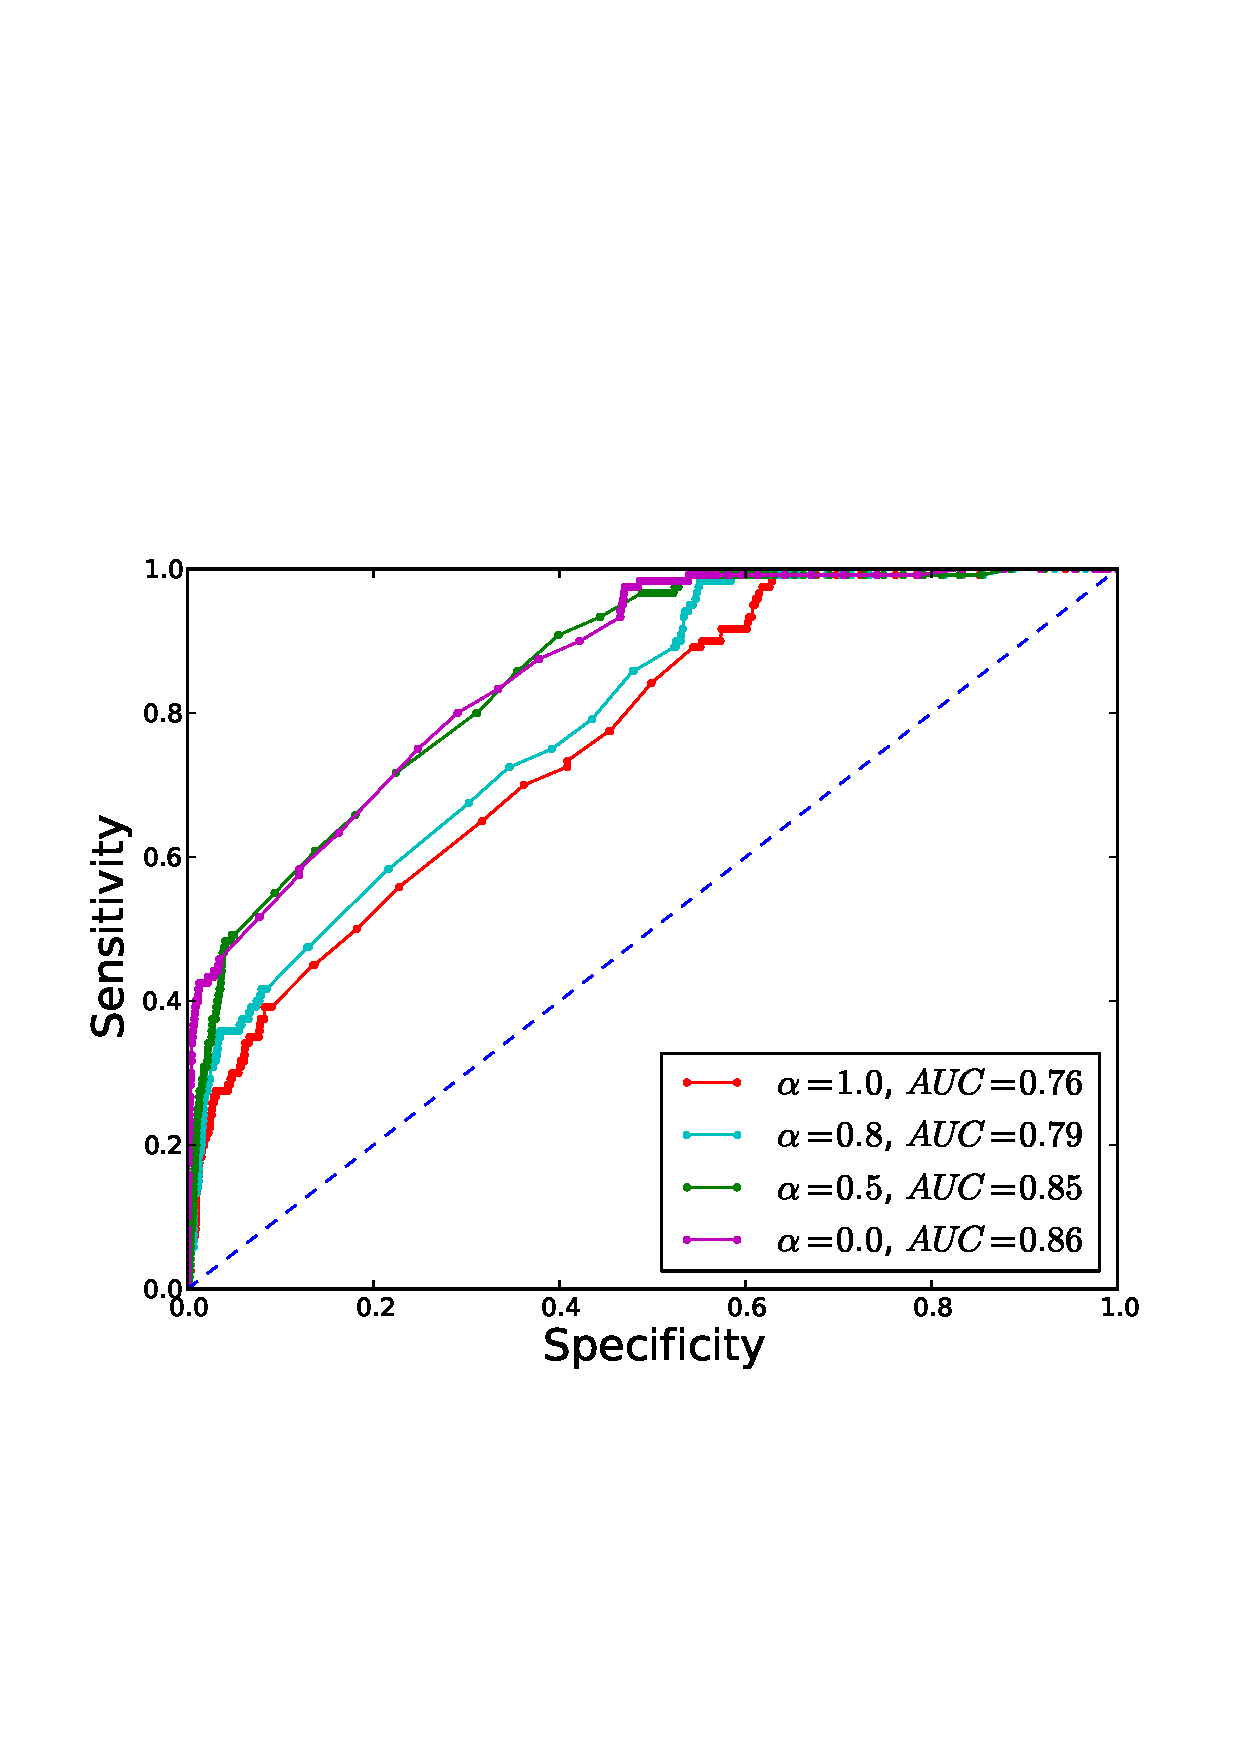
\includegraphics[width=1.2\textwidth]{figures/ROC_24.pdf}
%\caption{24 mutations}
%\label{fig:ROC24mut}
%\end{subfigure}
\caption{Performance of error-correction. Subfigures show accuracy with under-estimated error rates (6 mutations), exact estimates (12 mutations) and over estimates 
(24 mutations). We also analyze the impact of the parameter $\alpha$ distributing the weights of stacking pair energies vs isostericity scores and use values 
ranging of $\alpha=\{0,0.5,0.8,1.0\}$. The AUC is indicated in the legend of the figures. Each individual ROC curve represent the average performance over the 10 experiments.}
\label{fig:ROCall}\SpaceCheating
\end{figure}

Our data demonstrates that our algorithm exhibits interesting potential for error-correction applications. First, the AUC values (up to $0.86$) indicate that a
signal has been successfully extracted. This result has been achieved with errors in loop regions (i.e. without base pairing information) and thus suggests
that correction rates in structured regions (i.e. base paired regions) could be even higher. Next, the optimal values of $\alpha$ tend to be close to $0.0$. This 
finding suggests that, at this point, the information issued from the consideration of stacking energies is currently modest. However, specific examples showed improved performance
using this energy term. Further studies must be conducted to understand how to make the best use of it. Finally, our algorithm seems robust to the number of
presumed mutations. Indeed, good AUC values are achieved even with conservative estimates for the number of errors (c.f.~50\% of the errors, leading to 
Fig.~\ref{fig:ROCall}(a)), as well as with large  values (cf~200\% of the errors  in Fig.~\ref{fig:ROCall}(c)). It is worth noting that scoring schemes giving a larger weight on
the isostericity scores (i.e. for low $\alpha$ values) seem more robust to under- and over-estimating the number of errors.






%!TEX root = main_RNAPyro_JCB.tex
\section{Conclusion}
\label{sec:conclusion}

\TODOJerome{Etoffer la conclusion}
In this article we presented a new and efficient way of exploring the mutational landscape of an RNA under structural constraints,
and apply our techniques to identify and fix sequencing errors. In addition, we introduced a new scoring scheme to measure the
likelihood of sequencing errors that combines the classical nearest-neighbour energy model parameters \cite{Turner2010} to the recently introduced
isostericity matrices \cite{Stombaugh2009}. The latter accounting for geometrical discrepancies occurring during base pair replacements.
Importantly, our algorithm runs in  $\Theta(n\cdot(|\Omega|+M^2))$ time and $\Theta(n\cdot(|\Omega|+M))$ memory, where $n$ is the length of the RNA,
$M$ the number of mutations and $\Omega$ the size of the multiple sequence alignment. This achievement enables us to envision applications to high-throughput sequencing pipe-lines.


By combining these two approaches into \texttt{RNApyro} ,  the 
mutational landscape exploration and the pseudo energy model,
 we created a tool predicting the positions
 yielding point-wise sequencing error and correcting them.
We validated our model with the 5s rRNA,
as presented in Sec.~\ref{sec:results}.
We observed that the models
with larger weights on the
isostericity seems to hold a higher accuracy on the estimation of errors.
This indicates that an exploitable signal is captured by the isostericity.
Importantly, the implementation is fast enough for practical applications. 


We must recall that our approach is restricted to
 the correction of point-wise error in structured regions (i.e. base paired nucleotides).
 Nonetheless it should supplement well existing tools, by using previously discarded
information holding, as shown, a strong signal.

Further research, given the potential of error-correction of \texttt{RNApyro}, 
will evaluate its impact over large datasets with different existing
  NGS error-correction pipe-line.

%!TEX root = main_RNAPyro_JCB.tex
\section{Acknowledgments}
\label{sec:acknowledgments}
The authors would like to thank Rob Knight for his suggestions and comments.
This work was funded by the French Agence Nationale de la Recherche (ANR) through the {\sc Magnum} {\tt ANR 2010 BLAN 0204} 
project (to YP), the
FQRNT team grant 232983 (to VR and JW) and NSERC Discovery grant 219671 (to JW).
%\newpage

\bibliographystyle{jcompbiol}
\bibliography{RNApyro}


\end{document}  
